\chapter{Branching Modell}

Beim Branching Modell wurde ein Modell ähnlich dem Dezentralen Branching Modell verwendet. Im Zentrum steht der Master Branch welche den derzeitigen Stand aller fertig entwickelten Features enthält. Um das Zentrum herum gibt es Feature Branches in denen aktiv Features entwickelt und getestet werden. Untereinander tauschen diese Feature Branches auch ihre Änderungen aus. Ist eine Feature Branch fertig getestet und überprüft, wird sie in den Master Branch gemerged und geschlossen.

\begin{figure}[H]
	\centering
	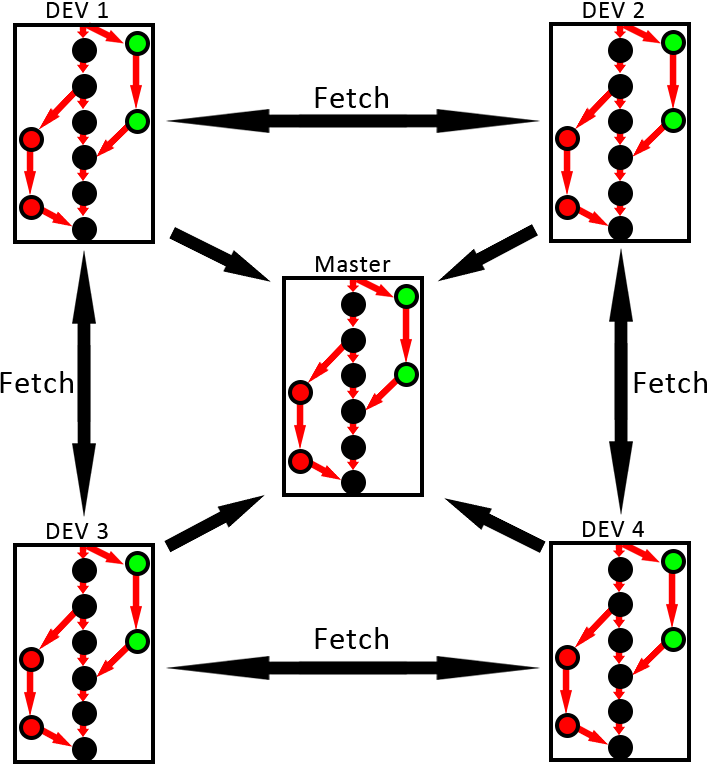
\includegraphics[width=0.7\textwidth]{branch/center_repo.png}
	\caption{Projekt Branching Modell}
	\label{figure:diagram_branching_model}
\end{figure}